\mysection{Úvod}

V našom ročníkovom projekte, sme sa rozhodli zaoberať vizualizáciou distribuovaných algortimov
pomocou Java aplikácie, ktorá umožňuje jednoduché a rýchle pochopenie tématu, bez
študovania dlhých odborných textov.

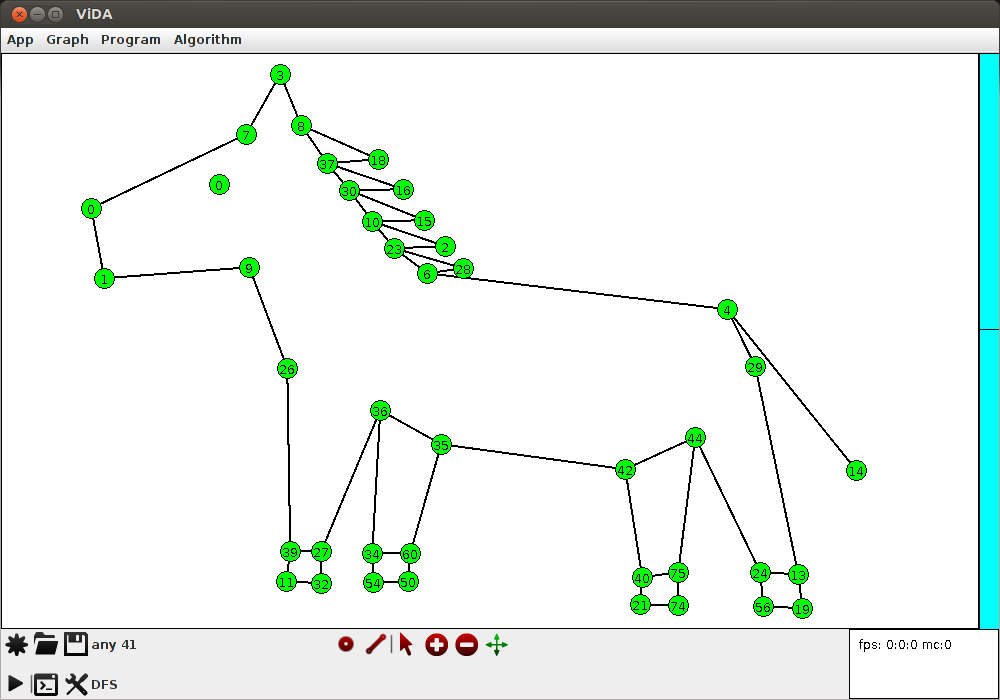
\includegraphics[width=\columnwidth]{konik}
%\caption{Vzhľad aplikácie po spustení}

\mysection{Hlavné ciele}
\begin{itemize}

    \item vizualizácie ušité na mieru konkrétnym distribuovaným algoritmov
    \item interaktivita s používateľom
    \item prehľadnosť a jednoduchosť používania aplikácie
    \item schopnosť vizualizovať vlastné algoritmy

\end{itemize}

